
\documentclass[compress]{beamer}

%\usepackage{beamerthemesplit}
\usepackage{xmpmulti}

\usepackage{graphicx,float,wrapfig, bbm}
\usepackage{amsfonts, bbold, comment}
\usepackage{mdwlist}
\usepackage{subfigure}
\usepackage{colortbl}

\usepackage{multirow}

\pgfdeclareimage[width=\paperwidth]{mybackground}{../../common/boulder.pdf}

\newcommand{\gfxs}[2]{
\begin{center}
	\includegraphics[width=#2\linewidth]{simtrans/#1}
\end{center}
}

\newcommand{\gfxq}[2]{
\begin{center}
	\includegraphics[width=#2\linewidth]{qb/#1}
\end{center}
}


\usetheme[pageofpages=of,                    % String used between the current page and the
                                             % total page count.
          bullet=circle,                     % Use circles instead of squares for bullets.
          titleline=true,                    % Show a line below the frame title.
          showdate=true,                     % show the date on the title page
          alternativetitlepage=true,         % Use the fancy title page.
          titlepagelogo=general_figures/culogo,              % Logo for the first page.
          % Logo for the header on first page.
          headerlogo=general_figures/boulder_cs,
          ]{UCBoulder}

\usecolortheme{ucdblack}
\title[Thinking on Your Feet]{Thinking on your Feet: Reinforcement Learning for Incremental
Language Tasks}
\author{ Jordan Boyd-Graber}
\date{Fall 2014}

\institute[Boulder] % (optional, but mostly needed)
{University of Colorado Boulder}

\AtBeginSection[] % "Beamer, do the following at the start of every section"
{ \begin{frame} \frametitle{Outline} % make a frame titled "Outline"
\tableofcontents[currentsection] % show TOC and highlight current section
\end{frame} }

\begin{document}

\frame{
\titlepage
\tiny
}


\begin{frame}{Nuremburg Trials}

\begin{columns}

\column{.5\linewidth}

    \gfxs{nuremberg_trials}{1.0}

\column{.5\linewidth}

    \begin{itemize}
        \item Dozens of defendants
        \item Judges from four nations (three languages)
     \end{itemize}

\end{columns}

\end{frame}


\begin{frame}{How Long are you Willing to Wait for a Translation?}

\begin{itemize}
  \item If you have to wait until the person speaking stops talking,
    then they wait for you to finish translating, it can take
    \emph{forever}!
    \pause
   \item Much better \only<3->{if you could get}
     \only<4->{translations as soon as possible}
\end{itemize}

\end{frame}


\begin{frame}{Algorithms that think on their feet}

\begin{columns}

  \column{.65\linewidth}
  \begin{itemize}
     \item Algorithms that process examples \emph{one word at a time}
       \begin{itemize}
         \item Simultaneous machine translation
         \item Trivia games
       \end{itemize}
      \item Similar structure
        \begin{itemize}
          \item Prediction
          \item Policy
        \end{itemize}
  \end{itemize}

  \column{.3\linewidth}

  \gfxs{nuremberg_translators}{.7}
  \gfxq{quizbowl}{.7}

\end{columns}

\end{frame}

\section{Simultaneous Translation}

\begin{frame}{Simultaneous translation is the norm}

  \begin{columns}
    \column{.5\linewidth}
       \gfxs{nuremberg_translators}{.9}
    \column{.5\linewidth}
       \begin{itemize}
         \item Rigorous training
         \item Technological sophistication
         \item Long way from ``sentence at a time''
       \end{itemize}
  \end{columns}

\end{frame}

\begin{frame}{Why simultaneous translation really hard is}

  \begin{columns}
    \column{.5\linewidth}
      \begin{itemize}
        \item Many languages are \textsc{sov}
        \item \alert<2>{German}, Japanese, Farsi, Korean, \alert<3>{Yiddish}
      \end{itemize}
    \column{.5\linewidth}
      \gfxs{yoda}{.6}
  \end{columns}

  \centering

\only<4->{
\vspace{1cm}

\begin{tabular}{c@{ }c@{ }c@{ }c@{ }c@{ }c@{ }c@{ }l}
ich & bin & mit & dem & Zug & nach & Ulm & {\bf gefahren} \\
I & am & with & the & train & to & Ulm & {\bf traveled} \\
\hline
I & \multicolumn{6}{c}{\emph{(\dots\dots waiting\dots\dots)}} & {\bf traveled} by train to Ulm \\
\end{tabular}
}

\end{frame}

\section{Quiz Bowl}

\begin{frame}
	\frametitle{Humans doing Incremental Classification}
	\begin{columns}

	\column{.5\linewidth}
	\begin{itemize}
		\item Game called ``quiz bowl''
		\item Two teams play each other
		\begin{itemize}
			\item Moderator reads a question
			\item When a team knows the answer, they signal (``buzz'' in)
			\item If right, they get points; otherwise, rest of the question is read to the other team
		\end{itemize}
		\item Hundreds of teams in the US alone
                \only<2>{\item Example \dots}
	\end{itemize}

	\column{.5\linewidth}
	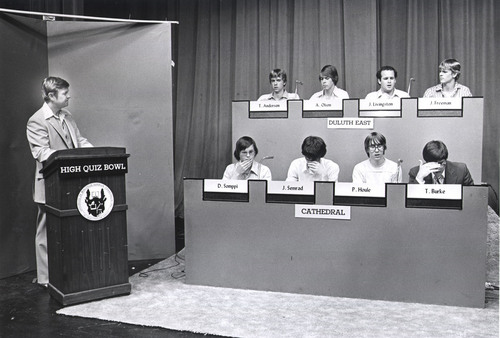
\includegraphics{qb/quizbowl}

	\end{columns}

\end{frame}

\begin{comment}

\begin{frame}[t]
	\frametitle{Sample Question 1}

With Leo Szilard, he invented a doubly-eponymous \only<2->{refrigerator with no moving parts. He did not take interaction with neighbors into account when formulating his theory of} \only<3->{heat capacity, so} \only<4->{Debye adjusted the theory for low temperatures. His} \only<4->{summation convention automatically sums repeated indices in tensor products. His name is attached to the A and B coefficients} \only<5->{for spontaneous and stimulated emission, the subject of one of his multiple groundbreaking 1905 papers. He further developed the model of statistics sent to him by} \only<6->{Bose to describe particles with integer spin. For 10 points, who is this German physicist best known for formulating the} \only<7->{special and general theories of relativity?} \\
\vspace{1cm}
\only<8->{ {\bf Albert \underline{Einstein}}}
\end{frame}

\end{comment}


\begin{frame}[t]
\frametitle{Sample Question}

One is Monte Carlo if at least half of the possible results for all x in a
\only<2->{language it says ``yes'' and ``no'' otherwise. One is called} \only<3->{unambiguous if for any $x$ there is at most one accepting computation. One is
called} \only<4->{oblivious if the position of the} \only<5->{cursor at the $t^{th}$
step depends only on the $t$ and the length of the input. One is} \only<6->{non-deterministic if its sets of next} \only<7->{states may contain more than one
element. For ten points, identify this model of} \only<8->{computation named for
an} \only<9->{English computer scientist.} \\
\only<10->{{\bf ANSWER: \underline{Turing} Machine (prompt on TM)}}


\end{frame}



\end{document}
